\section{Description de l'interface}
	\subsection{Menu principal}
		Le menu principal dispose de 4 options (cf \ref{fig:menuPrinc})
		
		\begin{description}
			\item[Nouvelle partie] \hfill \\
				Permet de créer une nouvelle partie à partir de paramètres. Repportez vous à la sous-section \ref{subsec:nouvellpartie} pour plus de détails.
			\item[Charger partie] \hfill \\
				Permet de charger une partie enregistrée. Repportez vous à la sous-section \ref{subsec:sauvergardes} pour plus de détails.
			\item[Regles du jeu] \hfill \\
				Bref rappel des rêgles du jeu. Une version plus complète est disponible dans la section \ref{sec:regles}.
			\item[Quitter] \hfill \\
				Fermeture de l'application et retour au bureau.
		\end{description}
		
		\begin{figure}[h!]
			\caption{Le menu principal}
			\label{fig:menuPrinc}
			\centering
			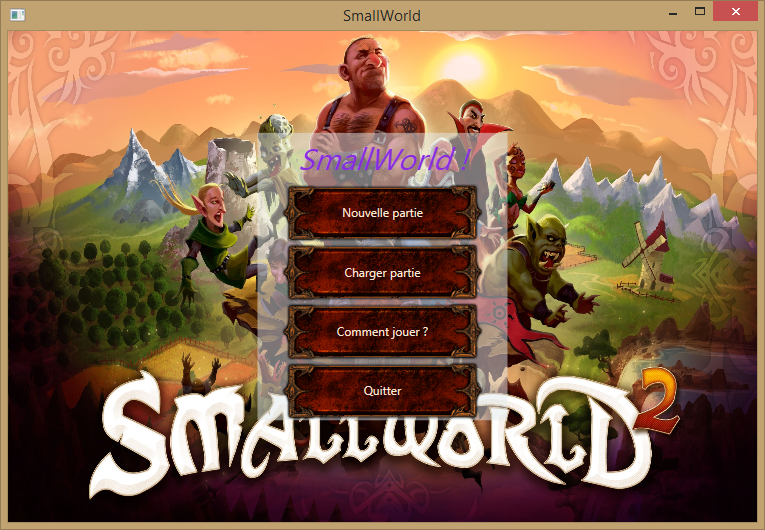
\includegraphics[width=\textwidth]{res/main_menu}
		\end{figure}
	
	\subsection{Menu nouvelle partie}
		\label{subsec:nouvellpartie}
		Toute création de partie passe par ce menu. Les joueurs doivent dabord choisir le type de carte, qui définira leur taille, le temps de jeu et le nombre d'unités de chaque joueur.
		Chaque joueur devra ensuite choisir un nom et un peuple. Deux joueurs ne peuvent évidement pas choisir le même peuple. Point de guerres fratricides dans Smallworld !
		Il ne reste plus qu'a cliquer sur \textit{Lancer la partie} pour commencer les hostilités.
		\begin{figure}[h!]
			\caption{Le menu de création de partie}
			\label{fig:menuCreat}
			\centering
			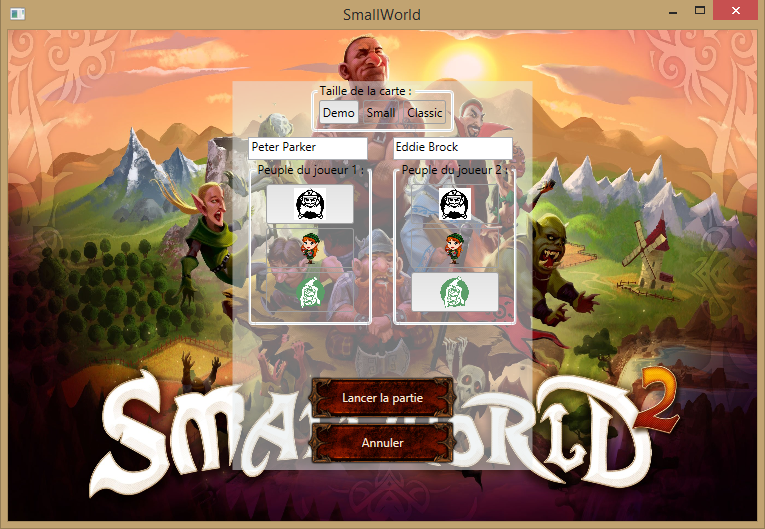
\includegraphics[width=\textwidth]{res/new_game}
		\end{figure}
		
	\subsection{Menu de gestion des sauvegardes}
		\label{subsec:sauvergardes}
		Ce menu permet de charger et sauvegarder les parties. Une partie sauvegardée peut être reprise dans les conditions identique à sa sauvegarde. Le tour, les points et les positions des unités sont inchangées.
		\begin{enumerate}
			\item \textsc{Liste des sauvegardes} : Toutes les parties enregistrées sont visibles dans ce cadre. Il est possible d'en sélectionner une avec un clic.
			\item \textsc{Zone de nommage de sauvegarde} : Dans le cas ou l'on désire créer une nouvelle sauvegarde, il est possible de rentrer son nom ici.
			\item \textsc{Bouton de chargement} : Permet de charger la partie sélectionnée dans la liste des sauvegardes.
			\item \textsc{Bouton de sauvegarde} : Permet d'enregistrer la partie en cours sous un nouveau nom ou à la place d'une ancienne sauvegarde, suivant ce qui est sélectionné. 
					Ce bouton est désactivé pour les utilisateurs provenant du menu principal.
			\item \textsc{Bouton de suppression de sauvegarde} : Permet de supprimer définitivement une sauvegarde sélectionnée dans la liste. attention, il n'y a aucun moyen de faire marche arrière !
			\item \textsc{Bouton de retour à l'écran précédent} : Permet de retourner à l'écran précédent, c'est à dire le menu principal ou le jeu.	
		\end{enumerate}
		
		\begin{figure}[h!]
			\caption{Le menu de sauvegarde et de chargement}
			\label{fig:menuCreat}
			\centering
			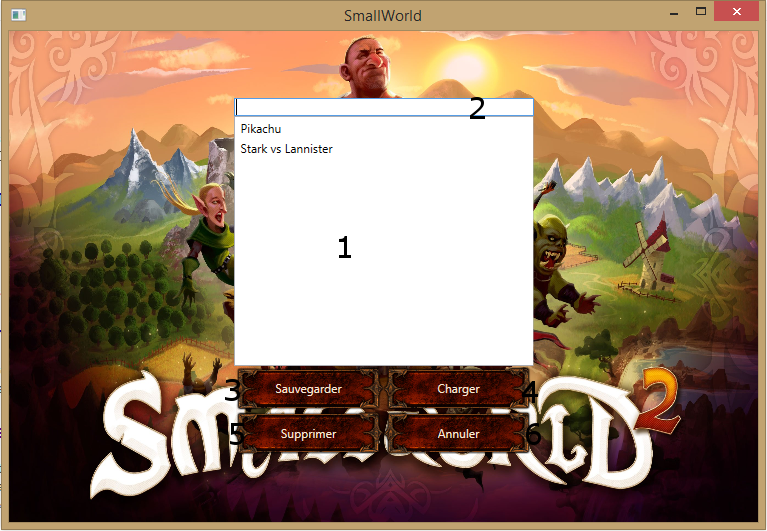
\includegraphics[width=\textwidth]{res/save_menu_annot}
		\end{figure}
		
	\subsection{Interface de jeu}
		\label{sec:interfaceIG}
		Les différentes fontionnalités de l'interface sont décrites ci dessous :
		\begin{enumerate}
			\item \textsc{Plateau de jeu} 
			\item \textsc{Curseur} : Permet de sélectionner les tuiles et les unités.
			\item \textsc{Score des joueurs} : Le joueur courant est indiqué en violet.
			\item \textsc{Etat du jeu} : Rappelle l'état des tours et le joueur courant.
			\item \textsc{Description de la tuile courante} : Donne son type, le nombre de points qu'elle donne et le cout pour s'y déplacer.
			\item \textsc{Description de l'unité courante} : Donne le nom, la vie actuelle, les points de mouvements restants, l'attaque et la défense de l'unité courante.
						Il est possible de changer d'unité avec les flèches sous le cadre.
			\item \textsc{Bouton de sauvegarde/chargement} : Ouvre le menu de gestion des sauvegardes, cf \ref{subsec:sauvergardes}.
			\item \textsc{Bouton de fin de tour} : Permet de finir le tour courant et de passer la main à son adversaire.
			\item \textsc{Abandonner} : Abandonne la partie en cours et retourne à l'écran titre.
		\end{enumerate}
		
		\begin{figure}[h!]
			\caption{Interface pendant le jeu}
			\label{fig:interfaceIG}
			\centering
			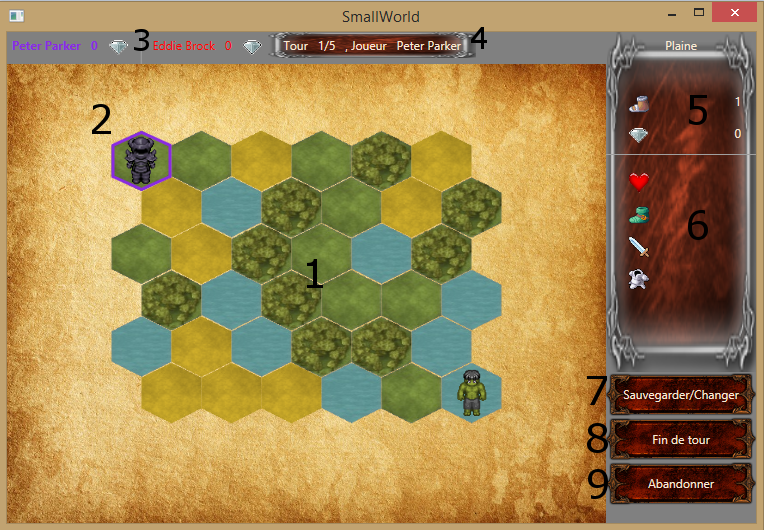
\includegraphics[width=\textwidth]{res/in_game_annot}
		\end{figure}
		
		Controles du jeu : 
		\begin{description}
			\item[Click gauche] \hfill \\
				Déplacement du curseur sur la carte.
			\item[Click droit] \hfill \\
				Déplacement de l'unité sélectionnée.
			\item[Espace] \hfill \\
				Unité suivante.
			\item[Entrée] \hfill \\
				Fin de tour.
			\item[Pavé numérique] \hfill \\
				Déplacement de l'unité sélectionnée. Les déplacements sont décrit sur le schéma \ref{fig:poskeys}
		\end{description}
		
		\begin{figure}[h!]
			\caption{Correspondance touche pavé numérique - déplacement}
			\label{fig:poskeys}
			\centering
			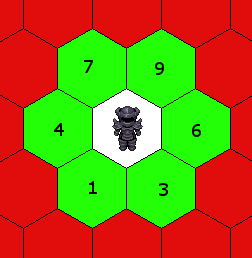
\includegraphics[width=0.5\textwidth]{res/pavnum_moves}
		\end{figure}
		
		Lorsque l'une des condition de fin de jeu est remplie, le jeu se termine et propose un tableau des scores qui indique le gagnant de la partie ! (cf figure \ref{fig:finjeu})
		\begin{figure}[h!]
			\caption{Ecran de fin de jeu}
			\label{fig:finjeu}
			\centering
			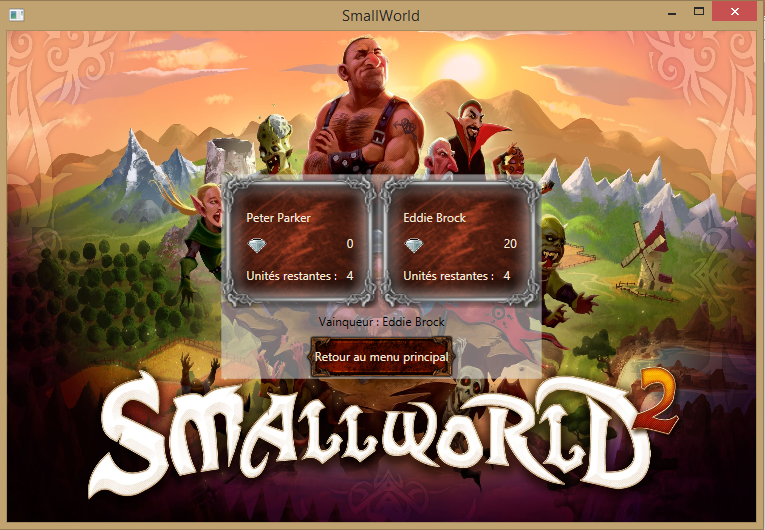
\includegraphics[width=\textwidth]{res/end_game}
		\end{figure}
